\documentclass[twoside]{book}

% Packages required by doxygen
\usepackage{fixltx2e}
\usepackage{calc}
\usepackage{doxygen}
\usepackage[export]{adjustbox} % also loads graphicx
\usepackage{graphicx}
\usepackage[utf8]{inputenc}
\usepackage{makeidx}
\usepackage{multicol}
\usepackage{multirow}
\PassOptionsToPackage{warn}{textcomp}
\usepackage{textcomp}
\usepackage[nointegrals]{wasysym}
\usepackage[table]{xcolor}

% NLS support packages
\usepackage[french]{babel}
\NoAutoSpaceBeforeFDP

% Font selection
\usepackage[T1]{fontenc}
\usepackage[scaled=.90]{helvet}
\usepackage{courier}
\usepackage{amssymb}
\usepackage{sectsty}
\renewcommand{\familydefault}{\sfdefault}
\allsectionsfont{%
  \fontseries{bc}\selectfont%
  \color{darkgray}%
}
\renewcommand{\DoxyLabelFont}{%
  \fontseries{bc}\selectfont%
  \color{darkgray}%
}
\newcommand{\+}{\discretionary{\mbox{\scriptsize$\hookleftarrow$}}{}{}}

% Page & text layout
\usepackage{geometry}
\geometry{%
  a4paper,%
  top=2.5cm,%
  bottom=2.5cm,%
  left=2.5cm,%
  right=2.5cm%
}
\tolerance=750
\hfuzz=15pt
\hbadness=750
\setlength{\emergencystretch}{15pt}
\setlength{\parindent}{0cm}
\setlength{\parskip}{3ex plus 2ex minus 2ex}
\makeatletter
\renewcommand{\paragraph}{%
  \@startsection{paragraph}{4}{0ex}{-1.0ex}{1.0ex}{%
    \normalfont\normalsize\bfseries\SS@parafont%
  }%
}
\renewcommand{\subparagraph}{%
  \@startsection{subparagraph}{5}{0ex}{-1.0ex}{1.0ex}{%
    \normalfont\normalsize\bfseries\SS@subparafont%
  }%
}
\makeatother

% Headers & footers
\usepackage{fancyhdr}
\pagestyle{fancyplain}
\fancyhead[LE]{\fancyplain{}{\bfseries\thepage}}
\fancyhead[CE]{\fancyplain{}{}}
\fancyhead[RE]{\fancyplain{}{\bfseries\leftmark}}
\fancyhead[LO]{\fancyplain{}{\bfseries\rightmark}}
\fancyhead[CO]{\fancyplain{}{}}
\fancyhead[RO]{\fancyplain{}{\bfseries\thepage}}
\fancyfoot[LE]{\fancyplain{}{}}
\fancyfoot[CE]{\fancyplain{}{}}
\fancyfoot[RE]{\fancyplain{}{\bfseries\scriptsize Généré par Doxygen }}
\fancyfoot[LO]{\fancyplain{}{\bfseries\scriptsize Généré par Doxygen }}
\fancyfoot[CO]{\fancyplain{}{}}
\fancyfoot[RO]{\fancyplain{}{}}
\renewcommand{\footrulewidth}{0.4pt}
\renewcommand{\chaptermark}[1]{%
  \markboth{#1}{}%
}
\renewcommand{\sectionmark}[1]{%
  \markright{\thesection\ #1}%
}

% Indices & bibliography
\usepackage{natbib}
\usepackage[titles]{tocloft}
\setcounter{tocdepth}{3}
\setcounter{secnumdepth}{5}
\makeindex

% Hyperlinks (required, but should be loaded last)
\usepackage{ifpdf}
\ifpdf
  \usepackage[pdftex,pagebackref=true]{hyperref}
\else
  \usepackage[ps2pdf,pagebackref=true]{hyperref}
\fi
\hypersetup{%
  colorlinks=true,%
  linkcolor=blue,%
  citecolor=blue,%
  unicode%
}

% Custom commands
\newcommand{\clearemptydoublepage}{%
  \newpage{\pagestyle{empty}\cleardoublepage}%
}

\usepackage{caption}
\captionsetup{labelsep=space,justification=centering,font={bf},singlelinecheck=off,skip=4pt,position=top}

%===== C O N T E N T S =====

\begin{document}

% Titlepage & ToC
\hypersetup{pageanchor=false,
             bookmarksnumbered=true,
             pdfencoding=unicode
            }
\pagenumbering{alph}
\begin{titlepage}
\vspace*{7cm}
\begin{center}%
{\Large S\+T\+O\+C\+K\+UP }\\
\vspace*{1cm}
{\large Généré par Doxygen 1.8.14}\\
\end{center}
\end{titlepage}
\clearemptydoublepage
\pagenumbering{roman}
\tableofcontents
\clearemptydoublepage
\pagenumbering{arabic}
\hypersetup{pageanchor=true}

%--- Begin generated contents ---
\chapter{Index hiérarchique}
\section{Class Hierarchy}
This inheritance list is sorted roughly, but not completely, alphabetically\+:\begin{DoxyCompactList}
\item \contentsline{section}{Base\+De\+Donnees}{\pageref{class_base_de_donnees}}{}
\item \contentsline{section}{Fournisseur}{\pageref{class_fournisseur}}{}
\item \contentsline{section}{Produits}{\pageref{class_produits}}{}
\item Q\+Dialog\begin{DoxyCompactList}
\item \contentsline{section}{Connexion}{\pageref{class_connexion}}{}
\end{DoxyCompactList}
\item Q\+Main\+Window\begin{DoxyCompactList}
\item \contentsline{section}{Main\+Window}{\pageref{class_main_window}}{}
\end{DoxyCompactList}
\item \contentsline{section}{Utilisateur}{\pageref{class_utilisateur}}{}
\end{DoxyCompactList}

\chapter{Index des classes}
\section{Liste des classes}
Liste des classes, structures, unions et interfaces avec une brève description \+:\begin{DoxyCompactList}
\item\contentsline{section}{\mbox{\hyperlink{class_base_de_donnees}{Base\+De\+Donnees}} \\*Interface vers fichier de base de données S\+Qlite3 }{\pageref{class_base_de_donnees}}{}
\item\contentsline{section}{\mbox{\hyperlink{class_connexion}{Connexion}} \\*Permet de gérer la connexion utilisateur }{\pageref{class_connexion}}{}
\item\contentsline{section}{\mbox{\hyperlink{class_fournisseur}{Fournisseur}} \\*Permet de gèrer les fournisseurs }{\pageref{class_fournisseur}}{}
\item\contentsline{section}{\mbox{\hyperlink{class_main_window}{Main\+Window}} \\*Permet de gèrer toutes les interactions dans la fenêtre principale }{\pageref{class_main_window}}{}
\item\contentsline{section}{\mbox{\hyperlink{class_produits}{Produits}} \\*Permet de gèrer les produits }{\pageref{class_produits}}{}
\item\contentsline{section}{\mbox{\hyperlink{class_utilisateur}{Utilisateur}} \\*Permet de gèrer les utilisateurs }{\pageref{class_utilisateur}}{}
\end{DoxyCompactList}

\chapter{Documentation des classes}
\hypertarget{class_base_de_donnees}{}\section{Référence de la classe Base\+De\+Donnees}
\label{class_base_de_donnees}\index{Base\+De\+Donnees@{Base\+De\+Donnees}}


Interface vers fichier de base de données S\+Qlite3.  




{\ttfamily \#include $<$basededonnees.\+h$>$}

\subsection*{Fonctions membres publiques}
\begin{DoxyCompactItemize}
\item 
\mbox{\Hypertarget{class_base_de_donnees_a888c0084f35395cc2aaae8326a27af06}\label{class_base_de_donnees_a888c0084f35395cc2aaae8326a27af06}} 
void \mbox{\hyperlink{class_base_de_donnees_a888c0084f35395cc2aaae8326a27af06}{creer\+Table\+Bdd}} ()
\begin{DoxyCompactList}\small\item\em creer\+Table\+Bdd Permet de créer les tables sql à l\textquotesingle{}installation de l\textquotesingle{}application \end{DoxyCompactList}\item 
\mbox{\Hypertarget{class_base_de_donnees_a635a8df387997ad54a4bcc4b8bce1a78}\label{class_base_de_donnees_a635a8df387997ad54a4bcc4b8bce1a78}} 
void \mbox{\hyperlink{class_base_de_donnees_a635a8df387997ad54a4bcc4b8bce1a78}{insertion\+Bdd\+Installation}} ()
\begin{DoxyCompactList}\small\item\em insertion\+Bdd\+Installation Permet de faire des insertion dans les tables de la base de données lors de l\textquotesingle{}installation de l\textquotesingle{}application \end{DoxyCompactList}\item 
void \mbox{\hyperlink{class_base_de_donnees_aaff06392cdd1aa3e3e66f1bb8214d1fb}{chercher\+Fournisseur}} (Q\+String trouver\+Fournisseur)
\begin{DoxyCompactList}\small\item\em chercher\+Fournisseur \end{DoxyCompactList}\item 
void \mbox{\hyperlink{class_base_de_donnees_a7741ad517714e619d7f8a0f202d3b38d}{chercher\+Produit\+Par\+Emplacement}} (Q\+Sql\+Query\+Model $\ast$model\+Chercher\+Produit\+Emplacement, Q\+String recherche\+Emplacement)
\begin{DoxyCompactList}\small\item\em chercher\+Produit\+Par\+Emplacement \end{DoxyCompactList}\item 
void \mbox{\hyperlink{class_base_de_donnees_a49d9a59025c2342adc820849bffb5532}{chercher\+Produit\+Par\+Nom}} (Q\+Sql\+Query\+Model $\ast$modelchercher\+Produit\+Par\+Nom, Q\+String chercher\+Produit\+Parnom)
\begin{DoxyCompactList}\small\item\em chercher\+Produit\+Par\+Nom \end{DoxyCompactList}\item 
bool \mbox{\hyperlink{class_base_de_donnees_a48345312e89c6e8fdeec128f033566ee}{creer\+Une\+Reference}} (\mbox{\hyperlink{class_produits}{Produits}} \&produit)
\begin{DoxyCompactList}\small\item\em creer\+Une\+Reference \end{DoxyCompactList}\item 
bool \mbox{\hyperlink{class_base_de_donnees_ae68726c99e17a89342655d8b842ced96}{mise\+Ajour\+Reference}} (\mbox{\hyperlink{class_produits}{Produits}} \&Mettre\+Ajour\+Produit)
\begin{DoxyCompactList}\small\item\em mise\+Ajour\+Reference \end{DoxyCompactList}\item 
bool \mbox{\hyperlink{class_base_de_donnees_a824bea64c3ef77eff0e4334a617b36c8}{supprimer\+Reference}} (\mbox{\hyperlink{class_produits}{Produits}} \&supprimer\+Produit)
\begin{DoxyCompactList}\small\item\em supprimer\+Reference \end{DoxyCompactList}\item 
bool \mbox{\hyperlink{class_base_de_donnees_acc7f10ab9b4699eaa495fa7829c0cfbd}{creer\+Un\+Utilisateur}} (\mbox{\hyperlink{class_utilisateur}{Utilisateur}} \&employe)
\begin{DoxyCompactList}\small\item\em creer\+Un\+Utilisateur \end{DoxyCompactList}\item 
\mbox{\Hypertarget{class_base_de_donnees_a9b8f8d9aca5ac268cba19329e3264c01}\label{class_base_de_donnees_a9b8f8d9aca5ac268cba19329e3264c01}} 
void \mbox{\hyperlink{class_base_de_donnees_a9b8f8d9aca5ac268cba19329e3264c01}{chercher\+Un\+Utilisateur}} ()
\begin{DoxyCompactList}\small\item\em chercher\+Un\+Utilisateur Permet de chercher un utilisateur dans la base de données \end{DoxyCompactList}\item 
bool \mbox{\hyperlink{class_base_de_donnees_a81715fc3632e6533d9c66a66c62e897b}{creer\+Un\+Fournisseur}} (\mbox{\hyperlink{class_fournisseur}{Fournisseur}} \&creer\+Fournisseur)
\begin{DoxyCompactList}\small\item\em creer\+Un\+Fournisseur \end{DoxyCompactList}\item 
bool \mbox{\hyperlink{class_base_de_donnees_ab49e6dfff0eecf616d9a7642ea358f31}{mise\+Ajour\+Fournisseur}} (\mbox{\hyperlink{class_fournisseur}{Fournisseur}} \&mettre\+Ajour\+Fournisseur)
\begin{DoxyCompactList}\small\item\em mise\+Ajour\+Fournisseur \end{DoxyCompactList}\item 
bool \mbox{\hyperlink{class_base_de_donnees_a4782a41060ec75d8343cb318b3b29a45}{supprimer\+Un\+Fournisseur}} (\mbox{\hyperlink{class_fournisseur}{Fournisseur}} \&supprimer\+Fournisseur)
\begin{DoxyCompactList}\small\item\em supprimer\+Un\+Fournisseur \end{DoxyCompactList}\item 
bool \mbox{\hyperlink{class_base_de_donnees_a9c2bce97f39046e66b3dd3d08c2b911a}{mise\+A\+Jour\+Utilisateur}} (\mbox{\hyperlink{class_utilisateur}{Utilisateur}} \&mettre\+Ajour\+Utilisateur)
\begin{DoxyCompactList}\small\item\em mise\+A\+Jour\+Utilisateur \end{DoxyCompactList}\item 
void \mbox{\hyperlink{class_base_de_donnees_a7ead23bc4e5d3bc897d9c6a412bbc0a6}{supprimer\+Un\+Utilisateur}} (\mbox{\hyperlink{class_utilisateur}{Utilisateur}} \&supprimer\+Utilisateur)
\begin{DoxyCompactList}\small\item\em supprimer\+Un\+Utilisateur \end{DoxyCompactList}\item 
\mbox{\Hypertarget{class_base_de_donnees_a1aa6b997245767e4ba75973d59dcfaf6}\label{class_base_de_donnees_a1aa6b997245767e4ba75973d59dcfaf6}} 
void \mbox{\hyperlink{class_base_de_donnees_a1aa6b997245767e4ba75973d59dcfaf6}{insertion\+En\+Bdd}} ()
\begin{DoxyCompactList}\small\item\em insertion\+En\+Bdd Execute la méthode qui fait l\textquotesingle{}insertion des données dans les tables lors de l\textquotesingle{}installation \end{DoxyCompactList}\item 
void \mbox{\hyperlink{class_base_de_donnees_aaa4a62ca5864ce24cb0b3d488a609811}{chercher\+Par\+Reference}} (Q\+Sql\+Query\+Model $\ast$model\+Chercher\+Par\+Reference, Q\+String search\+Ref)
\begin{DoxyCompactList}\small\item\em chercher\+Par\+Reference \end{DoxyCompactList}\end{DoxyCompactItemize}
\subsection*{Attributs publics}
\begin{DoxyCompactItemize}
\item 
\mbox{\Hypertarget{class_base_de_donnees_a2527e35f95ca7abc94d61eabe2b8ef17}\label{class_base_de_donnees_a2527e35f95ca7abc94d61eabe2b8ef17}} 
Q\+Sql\+Database \mbox{\hyperlink{class_base_de_donnees_a2527e35f95ca7abc94d61eabe2b8ef17}{stockup}}
\begin{DoxyCompactList}\small\item\em stockup \end{DoxyCompactList}\end{DoxyCompactItemize}


\subsection{Description détaillée}
Interface vers fichier de base de données S\+Qlite3. 

\subsection{Documentation des fonctions membres}
\mbox{\Hypertarget{class_base_de_donnees_aaff06392cdd1aa3e3e66f1bb8214d1fb}\label{class_base_de_donnees_aaff06392cdd1aa3e3e66f1bb8214d1fb}} 
\index{Base\+De\+Donnees@{Base\+De\+Donnees}!chercher\+Fournisseur@{chercher\+Fournisseur}}
\index{chercher\+Fournisseur@{chercher\+Fournisseur}!Base\+De\+Donnees@{Base\+De\+Donnees}}
\subsubsection{\texorpdfstring{chercher\+Fournisseur()}{chercherFournisseur()}}
{\footnotesize\ttfamily void Base\+De\+Donnees\+::chercher\+Fournisseur (\begin{DoxyParamCaption}\item[{Q\+String}]{trouver\+Fournisseur }\end{DoxyParamCaption})}



chercher\+Fournisseur 


\begin{DoxyParams}{Paramètres}
{\em trouver\+Fournisseur} & Permet d\textquotesingle{}effectuer la recherche d\textquotesingle{}un fournisseur \\
\hline
\end{DoxyParams}
\mbox{\Hypertarget{class_base_de_donnees_aaa4a62ca5864ce24cb0b3d488a609811}\label{class_base_de_donnees_aaa4a62ca5864ce24cb0b3d488a609811}} 
\index{Base\+De\+Donnees@{Base\+De\+Donnees}!chercher\+Par\+Reference@{chercher\+Par\+Reference}}
\index{chercher\+Par\+Reference@{chercher\+Par\+Reference}!Base\+De\+Donnees@{Base\+De\+Donnees}}
\subsubsection{\texorpdfstring{chercher\+Par\+Reference()}{chercherParReference()}}
{\footnotesize\ttfamily void Base\+De\+Donnees\+::chercher\+Par\+Reference (\begin{DoxyParamCaption}\item[{Q\+Sql\+Query\+Model $\ast$}]{model\+Chercher\+Par\+Reference,  }\item[{Q\+String}]{search\+Ref }\end{DoxyParamCaption})}



chercher\+Par\+Reference 


\begin{DoxyParams}{Paramètres}
{\em model\+Chercher\+Par\+Reference} & \\
\hline
{\em search\+Ref} & Permet de chercher une référence dans la base de donnée avec sa référence \\
\hline
\end{DoxyParams}
\mbox{\Hypertarget{class_base_de_donnees_a7741ad517714e619d7f8a0f202d3b38d}\label{class_base_de_donnees_a7741ad517714e619d7f8a0f202d3b38d}} 
\index{Base\+De\+Donnees@{Base\+De\+Donnees}!chercher\+Produit\+Par\+Emplacement@{chercher\+Produit\+Par\+Emplacement}}
\index{chercher\+Produit\+Par\+Emplacement@{chercher\+Produit\+Par\+Emplacement}!Base\+De\+Donnees@{Base\+De\+Donnees}}
\subsubsection{\texorpdfstring{chercher\+Produit\+Par\+Emplacement()}{chercherProduitParEmplacement()}}
{\footnotesize\ttfamily void Base\+De\+Donnees\+::chercher\+Produit\+Par\+Emplacement (\begin{DoxyParamCaption}\item[{Q\+Sql\+Query\+Model $\ast$}]{model\+Chercher\+Produit\+Emplacement,  }\item[{Q\+String}]{recherche\+Emplacement }\end{DoxyParamCaption})}



chercher\+Produit\+Par\+Emplacement 


\begin{DoxyParams}{Paramètres}
{\em model\+Chercher\+Produit\+Emplacement} & \\
\hline
{\em recherche\+Emplacement} & Permet de faire la recherche d\textquotesingle{}une matière première par emplacement \\
\hline
\end{DoxyParams}
\mbox{\Hypertarget{class_base_de_donnees_a49d9a59025c2342adc820849bffb5532}\label{class_base_de_donnees_a49d9a59025c2342adc820849bffb5532}} 
\index{Base\+De\+Donnees@{Base\+De\+Donnees}!chercher\+Produit\+Par\+Nom@{chercher\+Produit\+Par\+Nom}}
\index{chercher\+Produit\+Par\+Nom@{chercher\+Produit\+Par\+Nom}!Base\+De\+Donnees@{Base\+De\+Donnees}}
\subsubsection{\texorpdfstring{chercher\+Produit\+Par\+Nom()}{chercherProduitParNom()}}
{\footnotesize\ttfamily void Base\+De\+Donnees\+::chercher\+Produit\+Par\+Nom (\begin{DoxyParamCaption}\item[{Q\+Sql\+Query\+Model $\ast$}]{modelchercher\+Produit\+Par\+Nom,  }\item[{Q\+String}]{chercher\+Produit\+Parnom }\end{DoxyParamCaption})}



chercher\+Produit\+Par\+Nom 


\begin{DoxyParams}{Paramètres}
{\em modelchercher\+Produit\+Par\+Nom} & \\
\hline
{\em chercher\+Produit\+Parnom} & Permet de faire la recherche d\textquotesingle{}une matière première par nom \\
\hline
\end{DoxyParams}
\mbox{\Hypertarget{class_base_de_donnees_a48345312e89c6e8fdeec128f033566ee}\label{class_base_de_donnees_a48345312e89c6e8fdeec128f033566ee}} 
\index{Base\+De\+Donnees@{Base\+De\+Donnees}!creer\+Une\+Reference@{creer\+Une\+Reference}}
\index{creer\+Une\+Reference@{creer\+Une\+Reference}!Base\+De\+Donnees@{Base\+De\+Donnees}}
\subsubsection{\texorpdfstring{creer\+Une\+Reference()}{creerUneReference()}}
{\footnotesize\ttfamily bool Base\+De\+Donnees\+::creer\+Une\+Reference (\begin{DoxyParamCaption}\item[{\mbox{\hyperlink{class_produits}{Produits}} \&}]{produit }\end{DoxyParamCaption})}



creer\+Une\+Reference 


\begin{DoxyParams}{Paramètres}
{\em produit} & \\
\hline
\end{DoxyParams}
\begin{DoxyReturn}{Renvoie}
si l\textquotesingle{}opération en base de donnée s\textquotesingle{}est effectuée ou non. Permet de créer une nouvelle référence 
\end{DoxyReturn}
\mbox{\Hypertarget{class_base_de_donnees_a81715fc3632e6533d9c66a66c62e897b}\label{class_base_de_donnees_a81715fc3632e6533d9c66a66c62e897b}} 
\index{Base\+De\+Donnees@{Base\+De\+Donnees}!creer\+Un\+Fournisseur@{creer\+Un\+Fournisseur}}
\index{creer\+Un\+Fournisseur@{creer\+Un\+Fournisseur}!Base\+De\+Donnees@{Base\+De\+Donnees}}
\subsubsection{\texorpdfstring{creer\+Un\+Fournisseur()}{creerUnFournisseur()}}
{\footnotesize\ttfamily bool Base\+De\+Donnees\+::creer\+Un\+Fournisseur (\begin{DoxyParamCaption}\item[{\mbox{\hyperlink{class_fournisseur}{Fournisseur}} \&}]{creer\+Fournisseur }\end{DoxyParamCaption})}



creer\+Un\+Fournisseur 


\begin{DoxyParams}{Paramètres}
{\em creer\+Fournisseur} & \\
\hline
\end{DoxyParams}
\begin{DoxyReturn}{Renvoie}
si l\textquotesingle{}opération en base de donnée s\textquotesingle{}est effectuée ou non. Permet de créer un fournisseur 
\end{DoxyReturn}
\mbox{\Hypertarget{class_base_de_donnees_acc7f10ab9b4699eaa495fa7829c0cfbd}\label{class_base_de_donnees_acc7f10ab9b4699eaa495fa7829c0cfbd}} 
\index{Base\+De\+Donnees@{Base\+De\+Donnees}!creer\+Un\+Utilisateur@{creer\+Un\+Utilisateur}}
\index{creer\+Un\+Utilisateur@{creer\+Un\+Utilisateur}!Base\+De\+Donnees@{Base\+De\+Donnees}}
\subsubsection{\texorpdfstring{creer\+Un\+Utilisateur()}{creerUnUtilisateur()}}
{\footnotesize\ttfamily bool Base\+De\+Donnees\+::creer\+Un\+Utilisateur (\begin{DoxyParamCaption}\item[{\mbox{\hyperlink{class_utilisateur}{Utilisateur}} \&}]{employe }\end{DoxyParamCaption})}



creer\+Un\+Utilisateur 


\begin{DoxyParams}{Paramètres}
{\em employe} & \\
\hline
\end{DoxyParams}
\begin{DoxyReturn}{Renvoie}
si l\textquotesingle{}opération en base de donnée s\textquotesingle{}est effectuée ou non. Permet de créer un nouvel utilisateur 
\end{DoxyReturn}
\mbox{\Hypertarget{class_base_de_donnees_ab49e6dfff0eecf616d9a7642ea358f31}\label{class_base_de_donnees_ab49e6dfff0eecf616d9a7642ea358f31}} 
\index{Base\+De\+Donnees@{Base\+De\+Donnees}!mise\+Ajour\+Fournisseur@{mise\+Ajour\+Fournisseur}}
\index{mise\+Ajour\+Fournisseur@{mise\+Ajour\+Fournisseur}!Base\+De\+Donnees@{Base\+De\+Donnees}}
\subsubsection{\texorpdfstring{mise\+Ajour\+Fournisseur()}{miseAjourFournisseur()}}
{\footnotesize\ttfamily bool Base\+De\+Donnees\+::mise\+Ajour\+Fournisseur (\begin{DoxyParamCaption}\item[{\mbox{\hyperlink{class_fournisseur}{Fournisseur}} \&}]{mettre\+Ajour\+Fournisseur }\end{DoxyParamCaption})}



mise\+Ajour\+Fournisseur 


\begin{DoxyParams}{Paramètres}
{\em mettre\+Ajour\+Fournisseur} & \\
\hline
\end{DoxyParams}
\begin{DoxyReturn}{Renvoie}
si l\textquotesingle{}opération en base de donnée s\textquotesingle{}est effectuée ou non. Permet de mettre à jour un fournisseur 
\end{DoxyReturn}
\mbox{\Hypertarget{class_base_de_donnees_ae68726c99e17a89342655d8b842ced96}\label{class_base_de_donnees_ae68726c99e17a89342655d8b842ced96}} 
\index{Base\+De\+Donnees@{Base\+De\+Donnees}!mise\+Ajour\+Reference@{mise\+Ajour\+Reference}}
\index{mise\+Ajour\+Reference@{mise\+Ajour\+Reference}!Base\+De\+Donnees@{Base\+De\+Donnees}}
\subsubsection{\texorpdfstring{mise\+Ajour\+Reference()}{miseAjourReference()}}
{\footnotesize\ttfamily bool Base\+De\+Donnees\+::mise\+Ajour\+Reference (\begin{DoxyParamCaption}\item[{\mbox{\hyperlink{class_produits}{Produits}} \&}]{Mettre\+Ajour\+Produit }\end{DoxyParamCaption})}



mise\+Ajour\+Reference 


\begin{DoxyParams}{Paramètres}
{\em Mettre\+Ajour\+Produit} & \\
\hline
\end{DoxyParams}
\begin{DoxyReturn}{Renvoie}
si l\textquotesingle{}opération en base de donnée s\textquotesingle{}est effectuée ou non. Permet de faire la mise à jour d\textquotesingle{}une référence 
\end{DoxyReturn}
\mbox{\Hypertarget{class_base_de_donnees_a9c2bce97f39046e66b3dd3d08c2b911a}\label{class_base_de_donnees_a9c2bce97f39046e66b3dd3d08c2b911a}} 
\index{Base\+De\+Donnees@{Base\+De\+Donnees}!mise\+A\+Jour\+Utilisateur@{mise\+A\+Jour\+Utilisateur}}
\index{mise\+A\+Jour\+Utilisateur@{mise\+A\+Jour\+Utilisateur}!Base\+De\+Donnees@{Base\+De\+Donnees}}
\subsubsection{\texorpdfstring{mise\+A\+Jour\+Utilisateur()}{miseAJourUtilisateur()}}
{\footnotesize\ttfamily bool Base\+De\+Donnees\+::mise\+A\+Jour\+Utilisateur (\begin{DoxyParamCaption}\item[{\mbox{\hyperlink{class_utilisateur}{Utilisateur}} \&}]{mettre\+Ajour\+Utilisateur }\end{DoxyParamCaption})}



mise\+A\+Jour\+Utilisateur 


\begin{DoxyParams}{Paramètres}
{\em mettre\+Ajour\+Utilisateur} & \\
\hline
\end{DoxyParams}
\begin{DoxyReturn}{Renvoie}
si l\textquotesingle{}opération en base de donnée s\textquotesingle{}est effectuée ou non. Permet de mettre à jour un utilisateur 
\end{DoxyReturn}
\mbox{\Hypertarget{class_base_de_donnees_a824bea64c3ef77eff0e4334a617b36c8}\label{class_base_de_donnees_a824bea64c3ef77eff0e4334a617b36c8}} 
\index{Base\+De\+Donnees@{Base\+De\+Donnees}!supprimer\+Reference@{supprimer\+Reference}}
\index{supprimer\+Reference@{supprimer\+Reference}!Base\+De\+Donnees@{Base\+De\+Donnees}}
\subsubsection{\texorpdfstring{supprimer\+Reference()}{supprimerReference()}}
{\footnotesize\ttfamily bool Base\+De\+Donnees\+::supprimer\+Reference (\begin{DoxyParamCaption}\item[{\mbox{\hyperlink{class_produits}{Produits}} \&}]{supprimer\+Produit }\end{DoxyParamCaption})}



supprimer\+Reference 


\begin{DoxyParams}{Paramètres}
{\em supprimer\+Produit} & \\
\hline
\end{DoxyParams}
\begin{DoxyReturn}{Renvoie}
si l\textquotesingle{}opération en base de donnée s\textquotesingle{}est effectuée ou non. Permet de supprimer une référence 
\end{DoxyReturn}
\mbox{\Hypertarget{class_base_de_donnees_a4782a41060ec75d8343cb318b3b29a45}\label{class_base_de_donnees_a4782a41060ec75d8343cb318b3b29a45}} 
\index{Base\+De\+Donnees@{Base\+De\+Donnees}!supprimer\+Un\+Fournisseur@{supprimer\+Un\+Fournisseur}}
\index{supprimer\+Un\+Fournisseur@{supprimer\+Un\+Fournisseur}!Base\+De\+Donnees@{Base\+De\+Donnees}}
\subsubsection{\texorpdfstring{supprimer\+Un\+Fournisseur()}{supprimerUnFournisseur()}}
{\footnotesize\ttfamily bool Base\+De\+Donnees\+::supprimer\+Un\+Fournisseur (\begin{DoxyParamCaption}\item[{\mbox{\hyperlink{class_fournisseur}{Fournisseur}} \&}]{supprimer\+Fournisseur }\end{DoxyParamCaption})}



supprimer\+Un\+Fournisseur 


\begin{DoxyParams}{Paramètres}
{\em supprimer\+Un\+Fournisseur} & \\
\hline
\end{DoxyParams}
\begin{DoxyReturn}{Renvoie}
si l\textquotesingle{}opération en base de donnée s\textquotesingle{}est effectuée ou non. Permet de supprimer un fournisseur 
\end{DoxyReturn}
\mbox{\Hypertarget{class_base_de_donnees_a7ead23bc4e5d3bc897d9c6a412bbc0a6}\label{class_base_de_donnees_a7ead23bc4e5d3bc897d9c6a412bbc0a6}} 
\index{Base\+De\+Donnees@{Base\+De\+Donnees}!supprimer\+Un\+Utilisateur@{supprimer\+Un\+Utilisateur}}
\index{supprimer\+Un\+Utilisateur@{supprimer\+Un\+Utilisateur}!Base\+De\+Donnees@{Base\+De\+Donnees}}
\subsubsection{\texorpdfstring{supprimer\+Un\+Utilisateur()}{supprimerUnUtilisateur()}}
{\footnotesize\ttfamily void Base\+De\+Donnees\+::supprimer\+Un\+Utilisateur (\begin{DoxyParamCaption}\item[{\mbox{\hyperlink{class_utilisateur}{Utilisateur}} \&}]{supprimer\+Utilisateur }\end{DoxyParamCaption})}



supprimer\+Un\+Utilisateur 


\begin{DoxyParams}{Paramètres}
{\em supprimer\+Utilisateur} & Permet de supprimer un utilisateur \\
\hline
\end{DoxyParams}


La documentation de cette classe a été générée à partir des fichiers suivants \+:\begin{DoxyCompactItemize}
\item 
basededonnees.\+h\item 
basededonnees.\+cpp\end{DoxyCompactItemize}

\hypertarget{class_connexion}{}\section{Référence de la classe Connexion}
\label{class_connexion}\index{Connexion@{Connexion}}


Permet de gérer la connexion utilisateur.  




{\ttfamily \#include $<$connexion.\+h$>$}

Graphe d\textquotesingle{}héritage de Connexion\+:\begin{figure}[H]
\begin{center}
\leavevmode
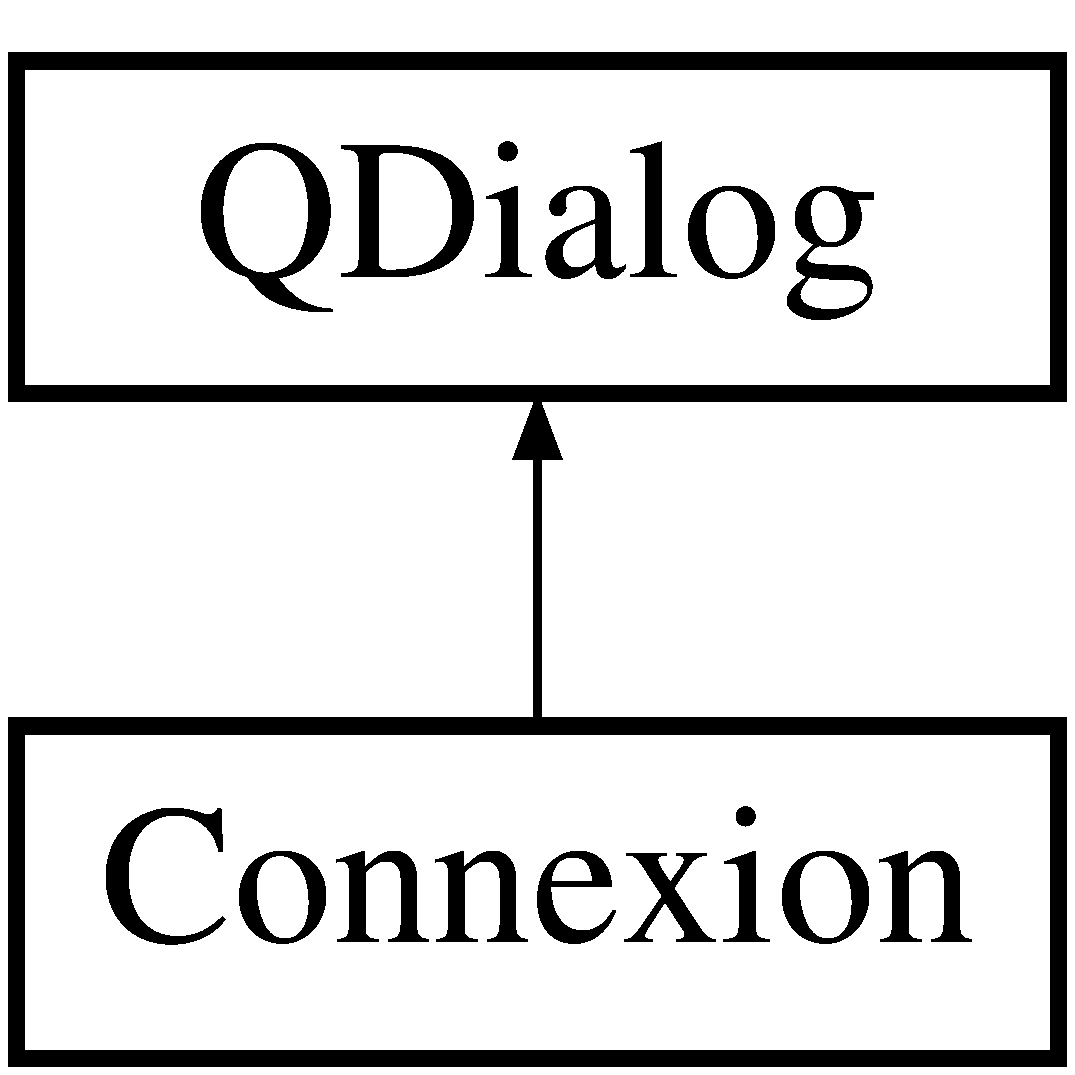
\includegraphics[height=2.000000cm]{class_connexion}
\end{center}
\end{figure}
\subsection*{Fonctions membres publiques}
\begin{DoxyCompactItemize}
\item 
\mbox{\Hypertarget{class_connexion_a5dc0e175fe7561fa4b1d206ec6f5db96}\label{class_connexion_a5dc0e175fe7561fa4b1d206ec6f5db96}} 
{\bfseries Connexion} (Q\+Widget $\ast$parent=0)
\item 
\mbox{\Hypertarget{class_connexion_ac06efdc729b3c51faf35c0e8b7e0fa7d}\label{class_connexion_ac06efdc729b3c51faf35c0e8b7e0fa7d}} 
void \mbox{\hyperlink{class_connexion_ac06efdc729b3c51faf35c0e8b7e0fa7d}{set\+Base\+De\+Donnees}} (\mbox{\hyperlink{class_base_de_donnees}{Base\+De\+Donnees}} $\ast$)
\begin{DoxyCompactList}\small\item\em set\+Base\+De\+Donnees \end{DoxyCompactList}\end{DoxyCompactItemize}
\subsection*{Attributs publics}
\begin{DoxyCompactItemize}
\item 
\mbox{\Hypertarget{class_connexion_a4ba4496266f3f38b57d7b413f2b7363f}\label{class_connexion_a4ba4496266f3f38b57d7b413f2b7363f}} 
\mbox{\hyperlink{class_utilisateur}{Utilisateur}} $\ast$ \mbox{\hyperlink{class_connexion_a4ba4496266f3f38b57d7b413f2b7363f}{carriste}}
\begin{DoxyCompactList}\small\item\em carriste \end{DoxyCompactList}\end{DoxyCompactItemize}


\subsection{Description détaillée}
Permet de gérer la connexion utilisateur. 

La documentation de cette classe a été générée à partir des fichiers suivants \+:\begin{DoxyCompactItemize}
\item 
connexion.\+h\item 
connexion.\+cpp\end{DoxyCompactItemize}

\hypertarget{class_fournisseur}{}\section{Référence de la classe Fournisseur}
\label{class_fournisseur}\index{Fournisseur@{Fournisseur}}


Permet de gèrer les fournisseurs.  




{\ttfamily \#include $<$fournisseur.\+h$>$}

\subsection*{Fonctions membres publiques}
\begin{DoxyCompactItemize}
\item 
\mbox{\hyperlink{class_fournisseur_a301b2476cc5f6f4c5ab220712dba8bf0}{Fournisseur}} (Q\+String id, Q\+String code\+Du\+Fournisseur, Q\+String nom\+Societe, Q\+String forme\+Juridique, Q\+String adresse, Q\+String code\+Postal, Q\+String ville, Q\+String pays, Q\+String telephone, Q\+String siret, Q\+String ape)
\begin{DoxyCompactList}\small\item\em \mbox{\hyperlink{class_fournisseur}{Fournisseur}}. \end{DoxyCompactList}\item 
Q\+String \mbox{\hyperlink{class_fournisseur_ae7ccf2a255b2ce31d88703dc5c28798d}{get\+Id\+Fournisseur}} ()
\begin{DoxyCompactList}\small\item\em get\+Id\+Fournisseur \end{DoxyCompactList}\item 
Q\+String \mbox{\hyperlink{class_fournisseur_a4ade53722bfbacf27e48f656ac74c6ee}{get\+Code\+Fournisseur}} ()
\begin{DoxyCompactList}\small\item\em get\+Code\+Fournisseur \end{DoxyCompactList}\item 
Q\+String \mbox{\hyperlink{class_fournisseur_ae83d27670f38c39d2ea4a3979e87c979}{get\+Nom\+Societe}} ()
\begin{DoxyCompactList}\small\item\em get\+Nom\+Societe \end{DoxyCompactList}\item 
Q\+String \mbox{\hyperlink{class_fournisseur_a5676a3819da9e28dbfc67f26f82ac9f5}{get\+Forme\+Juridique}} ()
\begin{DoxyCompactList}\small\item\em get\+Forme\+Juridique \end{DoxyCompactList}\item 
Q\+String \mbox{\hyperlink{class_fournisseur_a8f14d2c643575cc8bc7ce836d5bfe9bf}{get\+Adresse}} ()
\begin{DoxyCompactList}\small\item\em get\+Adresse \end{DoxyCompactList}\item 
Q\+String \mbox{\hyperlink{class_fournisseur_ab8daa4a60b7a40af956e40492ed249b8}{get\+Code\+Postal}} ()
\begin{DoxyCompactList}\small\item\em get\+Code\+Postal \end{DoxyCompactList}\item 
Q\+String \mbox{\hyperlink{class_fournisseur_ad526bb60f5bb68e79499244c6e174ac3}{get\+Ville}} ()
\begin{DoxyCompactList}\small\item\em get\+Ville \end{DoxyCompactList}\item 
Q\+String \mbox{\hyperlink{class_fournisseur_a5004e3d9666618fce013b58ef93b0560}{get\+Pays}} ()
\begin{DoxyCompactList}\small\item\em get\+Pays \end{DoxyCompactList}\item 
Q\+String \mbox{\hyperlink{class_fournisseur_af30a747841b0e07ffe42be13ccdf9066}{get\+Telephone}} ()
\begin{DoxyCompactList}\small\item\em get\+Telephone \end{DoxyCompactList}\item 
Q\+String \mbox{\hyperlink{class_fournisseur_a4194cdab5ed4dbcf97ac63369fa2be8d}{get\+Siret}} ()
\begin{DoxyCompactList}\small\item\em get\+Siret \end{DoxyCompactList}\item 
Q\+String \mbox{\hyperlink{class_fournisseur_aa85152c3305393fe49ba6a1480fcfea0}{get\+Ape}} ()
\begin{DoxyCompactList}\small\item\em get\+Ape \end{DoxyCompactList}\end{DoxyCompactItemize}


\subsection{Description détaillée}
Permet de gèrer les fournisseurs. 

\subsection{Documentation des constructeurs et destructeur}
\mbox{\Hypertarget{class_fournisseur_a301b2476cc5f6f4c5ab220712dba8bf0}\label{class_fournisseur_a301b2476cc5f6f4c5ab220712dba8bf0}} 
\index{Fournisseur@{Fournisseur}!Fournisseur@{Fournisseur}}
\index{Fournisseur@{Fournisseur}!Fournisseur@{Fournisseur}}
\subsubsection{\texorpdfstring{Fournisseur()}{Fournisseur()}}
{\footnotesize\ttfamily Fournisseur\+::\+Fournisseur (\begin{DoxyParamCaption}\item[{Q\+String}]{id,  }\item[{Q\+String}]{code\+Du\+Fournisseur,  }\item[{Q\+String}]{nom\+Societe,  }\item[{Q\+String}]{forme\+Juridique,  }\item[{Q\+String}]{adresse,  }\item[{Q\+String}]{code\+Postal,  }\item[{Q\+String}]{ville,  }\item[{Q\+String}]{pays,  }\item[{Q\+String}]{telephone,  }\item[{Q\+String}]{siret,  }\item[{Q\+String}]{ape }\end{DoxyParamCaption})}



\mbox{\hyperlink{class_fournisseur}{Fournisseur}}. 


\begin{DoxyParams}{Paramètres}
{\em id} & \\
\hline
{\em code\+Du\+Fournisseur} & \\
\hline
{\em nom\+Societe} & \\
\hline
{\em forme\+Juridique} & \\
\hline
{\em adresse} & \\
\hline
{\em code\+Postal} & \\
\hline
{\em ville} & \\
\hline
{\em pays} & \\
\hline
{\em telephone} & \\
\hline
{\em siret} & \\
\hline
{\em ape} & \\
\hline
\end{DoxyParams}


\subsection{Documentation des fonctions membres}
\mbox{\Hypertarget{class_fournisseur_a8f14d2c643575cc8bc7ce836d5bfe9bf}\label{class_fournisseur_a8f14d2c643575cc8bc7ce836d5bfe9bf}} 
\index{Fournisseur@{Fournisseur}!get\+Adresse@{get\+Adresse}}
\index{get\+Adresse@{get\+Adresse}!Fournisseur@{Fournisseur}}
\subsubsection{\texorpdfstring{get\+Adresse()}{getAdresse()}}
{\footnotesize\ttfamily Q\+String Fournisseur\+::get\+Adresse (\begin{DoxyParamCaption}{ }\end{DoxyParamCaption})}



get\+Adresse 

\begin{DoxyReturn}{Renvoie}
l\textquotesingle{}adresse 
\end{DoxyReturn}
\mbox{\Hypertarget{class_fournisseur_aa85152c3305393fe49ba6a1480fcfea0}\label{class_fournisseur_aa85152c3305393fe49ba6a1480fcfea0}} 
\index{Fournisseur@{Fournisseur}!get\+Ape@{get\+Ape}}
\index{get\+Ape@{get\+Ape}!Fournisseur@{Fournisseur}}
\subsubsection{\texorpdfstring{get\+Ape()}{getApe()}}
{\footnotesize\ttfamily Q\+String Fournisseur\+::get\+Ape (\begin{DoxyParamCaption}{ }\end{DoxyParamCaption})}



get\+Ape 

\begin{DoxyReturn}{Renvoie}
le code A\+PE 
\end{DoxyReturn}
\mbox{\Hypertarget{class_fournisseur_a4ade53722bfbacf27e48f656ac74c6ee}\label{class_fournisseur_a4ade53722bfbacf27e48f656ac74c6ee}} 
\index{Fournisseur@{Fournisseur}!get\+Code\+Fournisseur@{get\+Code\+Fournisseur}}
\index{get\+Code\+Fournisseur@{get\+Code\+Fournisseur}!Fournisseur@{Fournisseur}}
\subsubsection{\texorpdfstring{get\+Code\+Fournisseur()}{getCodeFournisseur()}}
{\footnotesize\ttfamily Q\+String Fournisseur\+::get\+Code\+Fournisseur (\begin{DoxyParamCaption}{ }\end{DoxyParamCaption})}



get\+Code\+Fournisseur 

\begin{DoxyReturn}{Renvoie}
le code fournisseur 
\end{DoxyReturn}
\mbox{\Hypertarget{class_fournisseur_ab8daa4a60b7a40af956e40492ed249b8}\label{class_fournisseur_ab8daa4a60b7a40af956e40492ed249b8}} 
\index{Fournisseur@{Fournisseur}!get\+Code\+Postal@{get\+Code\+Postal}}
\index{get\+Code\+Postal@{get\+Code\+Postal}!Fournisseur@{Fournisseur}}
\subsubsection{\texorpdfstring{get\+Code\+Postal()}{getCodePostal()}}
{\footnotesize\ttfamily Q\+String Fournisseur\+::get\+Code\+Postal (\begin{DoxyParamCaption}{ }\end{DoxyParamCaption})}



get\+Code\+Postal 

\begin{DoxyReturn}{Renvoie}
le code postal 
\end{DoxyReturn}
\mbox{\Hypertarget{class_fournisseur_a5676a3819da9e28dbfc67f26f82ac9f5}\label{class_fournisseur_a5676a3819da9e28dbfc67f26f82ac9f5}} 
\index{Fournisseur@{Fournisseur}!get\+Forme\+Juridique@{get\+Forme\+Juridique}}
\index{get\+Forme\+Juridique@{get\+Forme\+Juridique}!Fournisseur@{Fournisseur}}
\subsubsection{\texorpdfstring{get\+Forme\+Juridique()}{getFormeJuridique()}}
{\footnotesize\ttfamily Q\+String Fournisseur\+::get\+Forme\+Juridique (\begin{DoxyParamCaption}{ }\end{DoxyParamCaption})}



get\+Forme\+Juridique 

\begin{DoxyReturn}{Renvoie}
la forme juridique 
\end{DoxyReturn}
\mbox{\Hypertarget{class_fournisseur_ae7ccf2a255b2ce31d88703dc5c28798d}\label{class_fournisseur_ae7ccf2a255b2ce31d88703dc5c28798d}} 
\index{Fournisseur@{Fournisseur}!get\+Id\+Fournisseur@{get\+Id\+Fournisseur}}
\index{get\+Id\+Fournisseur@{get\+Id\+Fournisseur}!Fournisseur@{Fournisseur}}
\subsubsection{\texorpdfstring{get\+Id\+Fournisseur()}{getIdFournisseur()}}
{\footnotesize\ttfamily Q\+String Fournisseur\+::get\+Id\+Fournisseur (\begin{DoxyParamCaption}{ }\end{DoxyParamCaption})}



get\+Id\+Fournisseur 

\begin{DoxyReturn}{Renvoie}
l\textquotesingle{}id du fournisseur 
\end{DoxyReturn}
\mbox{\Hypertarget{class_fournisseur_ae83d27670f38c39d2ea4a3979e87c979}\label{class_fournisseur_ae83d27670f38c39d2ea4a3979e87c979}} 
\index{Fournisseur@{Fournisseur}!get\+Nom\+Societe@{get\+Nom\+Societe}}
\index{get\+Nom\+Societe@{get\+Nom\+Societe}!Fournisseur@{Fournisseur}}
\subsubsection{\texorpdfstring{get\+Nom\+Societe()}{getNomSociete()}}
{\footnotesize\ttfamily Q\+String Fournisseur\+::get\+Nom\+Societe (\begin{DoxyParamCaption}{ }\end{DoxyParamCaption})}



get\+Nom\+Societe 

\begin{DoxyReturn}{Renvoie}
le nom de la société 
\end{DoxyReturn}
\mbox{\Hypertarget{class_fournisseur_a5004e3d9666618fce013b58ef93b0560}\label{class_fournisseur_a5004e3d9666618fce013b58ef93b0560}} 
\index{Fournisseur@{Fournisseur}!get\+Pays@{get\+Pays}}
\index{get\+Pays@{get\+Pays}!Fournisseur@{Fournisseur}}
\subsubsection{\texorpdfstring{get\+Pays()}{getPays()}}
{\footnotesize\ttfamily Q\+String Fournisseur\+::get\+Pays (\begin{DoxyParamCaption}{ }\end{DoxyParamCaption})}



get\+Pays 

\begin{DoxyReturn}{Renvoie}
le pays 
\end{DoxyReturn}
\mbox{\Hypertarget{class_fournisseur_a4194cdab5ed4dbcf97ac63369fa2be8d}\label{class_fournisseur_a4194cdab5ed4dbcf97ac63369fa2be8d}} 
\index{Fournisseur@{Fournisseur}!get\+Siret@{get\+Siret}}
\index{get\+Siret@{get\+Siret}!Fournisseur@{Fournisseur}}
\subsubsection{\texorpdfstring{get\+Siret()}{getSiret()}}
{\footnotesize\ttfamily Q\+String Fournisseur\+::get\+Siret (\begin{DoxyParamCaption}{ }\end{DoxyParamCaption})}



get\+Siret 

\begin{DoxyReturn}{Renvoie}
le numéro de S\+I\+R\+ET 
\end{DoxyReturn}
\mbox{\Hypertarget{class_fournisseur_af30a747841b0e07ffe42be13ccdf9066}\label{class_fournisseur_af30a747841b0e07ffe42be13ccdf9066}} 
\index{Fournisseur@{Fournisseur}!get\+Telephone@{get\+Telephone}}
\index{get\+Telephone@{get\+Telephone}!Fournisseur@{Fournisseur}}
\subsubsection{\texorpdfstring{get\+Telephone()}{getTelephone()}}
{\footnotesize\ttfamily Q\+String Fournisseur\+::get\+Telephone (\begin{DoxyParamCaption}{ }\end{DoxyParamCaption})}



get\+Telephone 

\begin{DoxyReturn}{Renvoie}
le numéro de téléphone 
\end{DoxyReturn}
\mbox{\Hypertarget{class_fournisseur_ad526bb60f5bb68e79499244c6e174ac3}\label{class_fournisseur_ad526bb60f5bb68e79499244c6e174ac3}} 
\index{Fournisseur@{Fournisseur}!get\+Ville@{get\+Ville}}
\index{get\+Ville@{get\+Ville}!Fournisseur@{Fournisseur}}
\subsubsection{\texorpdfstring{get\+Ville()}{getVille()}}
{\footnotesize\ttfamily Q\+String Fournisseur\+::get\+Ville (\begin{DoxyParamCaption}{ }\end{DoxyParamCaption})}



get\+Ville 

\begin{DoxyReturn}{Renvoie}
la ville 
\end{DoxyReturn}


La documentation de cette classe a été générée à partir des fichiers suivants \+:\begin{DoxyCompactItemize}
\item 
fournisseur.\+h\item 
fournisseur.\+cpp\end{DoxyCompactItemize}

\hypertarget{class_main_window}{}\section{Référence de la classe Main\+Window}
\label{class_main_window}\index{Main\+Window@{Main\+Window}}


Permet de gèrer toutes les interactions dans la fenêtre principale.  




{\ttfamily \#include $<$mainwindow.\+h$>$}

Graphe d\textquotesingle{}héritage de Main\+Window\+:\begin{figure}[H]
\begin{center}
\leavevmode
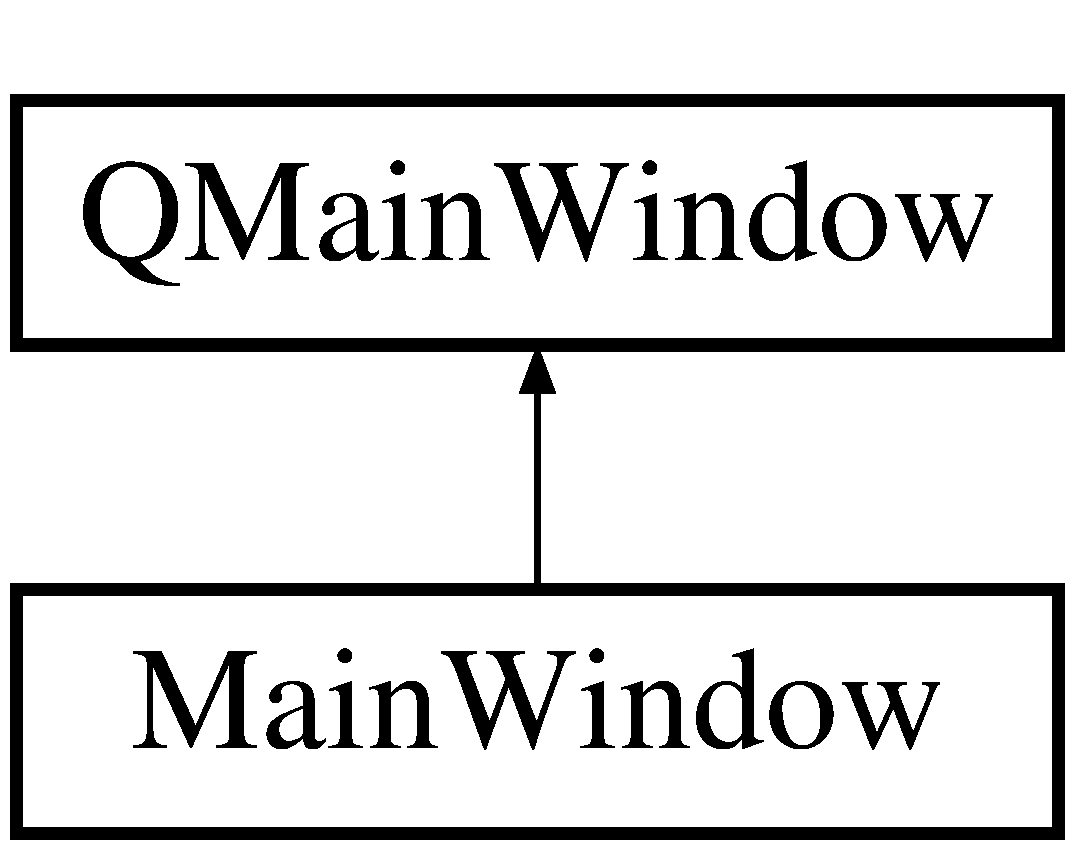
\includegraphics[height=2.000000cm]{class_main_window}
\end{center}
\end{figure}
\subsection*{Connecteurs publics}
\begin{DoxyCompactItemize}
\item 
\mbox{\Hypertarget{class_main_window_a5b477f0785cfed5fdffcda39ad7b92cb}\label{class_main_window_a5b477f0785cfed5fdffcda39ad7b92cb}} 
void \mbox{\hyperlink{class_main_window_a5b477f0785cfed5fdffcda39ad7b92cb}{desactiver\+Onglets\+Groupe\+Carriste}} ()
\begin{DoxyCompactList}\small\item\em desactiver\+Onglets\+Groupe\+Carriste Liste les différents onglets désactivés pour le groupe carriste \end{DoxyCompactList}\item 
\mbox{\Hypertarget{class_main_window_afe9d9d46e61e2460e636619577a9e8fd}\label{class_main_window_afe9d9d46e61e2460e636619577a9e8fd}} 
void \mbox{\hyperlink{class_main_window_afe9d9d46e61e2460e636619577a9e8fd}{on\+\_\+action\+Quitter\+\_\+triggered}} ()
\begin{DoxyCompactList}\small\item\em on\+\_\+action\+Quitter\+\_\+triggered Permet de fermer l\textquotesingle{}application \end{DoxyCompactList}\item 
\mbox{\Hypertarget{class_main_window_af416c87932d9675ef70ea737ad4b1a86}\label{class_main_window_af416c87932d9675ef70ea737ad4b1a86}} 
void \mbox{\hyperlink{class_main_window_af416c87932d9675ef70ea737ad4b1a86}{on\+\_\+action\+Vider\+\_\+la\+\_\+bas\+\_\+de\+\_\+donn\+\_\+es\+\_\+triggered}} ()
\begin{DoxyCompactList}\small\item\em on\+\_\+action\+Vider\+\_\+la\+\_\+bas\+\_\+de\+\_\+donn\+\_\+es\+\_\+triggered Permet de purger la table matieres\+\_\+\+Premieres et Fournisseurs. \end{DoxyCompactList}\item 
\mbox{\Hypertarget{class_main_window_a720083a9a815c386b46003d02b4034da}\label{class_main_window_a720083a9a815c386b46003d02b4034da}} 
void \mbox{\hyperlink{class_main_window_a720083a9a815c386b46003d02b4034da}{desactiver\+Onglets\+Groupe\+Qualite}} ()
\begin{DoxyCompactList}\small\item\em desactiver\+Onglets\+Groupe\+Qualite Liste les différents onglets désactivés pour le groupe labo qualite \end{DoxyCompactList}\item 
void \mbox{\hyperlink{class_main_window_a37382033fa3cefb818a17d198707abe1}{on\+\_\+list\+Database\+\_\+activated}} (const Q\+Model\+Index \&index)
\begin{DoxyCompactList}\small\item\em on\+\_\+list\+Database\+\_\+activated \end{DoxyCompactList}\item 
void \mbox{\hyperlink{class_main_window_a5c37de425b15bf9117aae7b6b67df243}{on\+\_\+list\+Provider\+\_\+activated}} (const Q\+Model\+Index \&index)
\begin{DoxyCompactList}\small\item\em on\+\_\+list\+Provider\+\_\+activated \end{DoxyCompactList}\item 
void \mbox{\hyperlink{class_main_window_a9c3a8c1df5ed2f93b79333aeab5a3323}{on\+\_\+gestion\+Utilisateur\+\_\+activated}} (const Q\+Model\+Index \&index)
\begin{DoxyCompactList}\small\item\em on\+\_\+gestion\+Utilisateur\+\_\+activated \end{DoxyCompactList}\end{DoxyCompactItemize}
\subsection*{Fonctions membres publiques}
\begin{DoxyCompactItemize}
\item 
\mbox{\Hypertarget{class_main_window_a8b244be8b7b7db1b08de2a2acb9409db}\label{class_main_window_a8b244be8b7b7db1b08de2a2acb9409db}} 
{\bfseries Main\+Window} (Q\+Widget $\ast$parent=0)
\item 
\mbox{\Hypertarget{class_main_window_a819bd562262c9bc43627a54b6748c0c4}\label{class_main_window_a819bd562262c9bc43627a54b6748c0c4}} 
void \mbox{\hyperlink{class_main_window_a819bd562262c9bc43627a54b6748c0c4}{set\+Base\+De\+Donnees}} (\mbox{\hyperlink{class_base_de_donnees}{Base\+De\+Donnees}} $\ast$)
\begin{DoxyCompactList}\small\item\em set\+Base\+De\+Donnees \end{DoxyCompactList}\item 
\mbox{\Hypertarget{class_main_window_ad98be47de90e967d8b5a51b4815f4c94}\label{class_main_window_ad98be47de90e967d8b5a51b4815f4c94}} 
void \mbox{\hyperlink{class_main_window_ad98be47de90e967d8b5a51b4815f4c94}{move\+To\+Tab}} (int)
\begin{DoxyCompactList}\small\item\em move\+To\+Tab \end{DoxyCompactList}\item 
\mbox{\Hypertarget{class_main_window_a025e31af5d47a5b1b448e52631d4e369}\label{class_main_window_a025e31af5d47a5b1b448e52631d4e369}} 
void \mbox{\hyperlink{class_main_window_a025e31af5d47a5b1b448e52631d4e369}{desactiver\+Onglet}} (int)
\begin{DoxyCompactList}\small\item\em disable\+Tab Permet de désactiver les onglet en fonction des droits utilisateurs \end{DoxyCompactList}\item 
Q\+String \mbox{\hyperlink{class_main_window_ab960f7157f5e796f4d4aa8e4d33ce4a9}{date\+Creation}} ()
\begin{DoxyCompactList}\small\item\em date\+Creation \end{DoxyCompactList}\item 
Q\+String \mbox{\hyperlink{class_main_window_a67ddd81f2fe064ae24dd662f06111230}{heure}} ()
\begin{DoxyCompactList}\small\item\em heure \end{DoxyCompactList}\end{DoxyCompactItemize}
\subsection*{Attributs publics}
\begin{DoxyCompactItemize}
\item 
\mbox{\Hypertarget{class_main_window_afcb22251b55d008d21b1889bab07863d}\label{class_main_window_afcb22251b55d008d21b1889bab07863d}} 
\mbox{\hyperlink{class_utilisateur}{Utilisateur}} $\ast$ \mbox{\hyperlink{class_main_window_afcb22251b55d008d21b1889bab07863d}{carriste}}
\begin{DoxyCompactList}\small\item\em carriste \end{DoxyCompactList}\end{DoxyCompactItemize}


\subsection{Description détaillée}
Permet de gèrer toutes les interactions dans la fenêtre principale. 

\subsection{Documentation des fonctions membres}
\mbox{\Hypertarget{class_main_window_ab960f7157f5e796f4d4aa8e4d33ce4a9}\label{class_main_window_ab960f7157f5e796f4d4aa8e4d33ce4a9}} 
\index{Main\+Window@{Main\+Window}!date\+Creation@{date\+Creation}}
\index{date\+Creation@{date\+Creation}!Main\+Window@{Main\+Window}}
\subsubsection{\texorpdfstring{date\+Creation()}{dateCreation()}}
{\footnotesize\ttfamily Q\+String Main\+Window\+::date\+Creation (\begin{DoxyParamCaption}{ }\end{DoxyParamCaption})}



date\+Creation 

\begin{DoxyReturn}{Renvoie}
la date du système Permet d\textquotesingle{}obtenir la date du système 
\end{DoxyReturn}
\mbox{\Hypertarget{class_main_window_a67ddd81f2fe064ae24dd662f06111230}\label{class_main_window_a67ddd81f2fe064ae24dd662f06111230}} 
\index{Main\+Window@{Main\+Window}!heure@{heure}}
\index{heure@{heure}!Main\+Window@{Main\+Window}}
\subsubsection{\texorpdfstring{heure()}{heure()}}
{\footnotesize\ttfamily Q\+String Main\+Window\+::heure (\begin{DoxyParamCaption}{ }\end{DoxyParamCaption})}



heure 

\begin{DoxyReturn}{Renvoie}
l\textquotesingle{}heure du système Permet d\textquotesingle{}obtenir l\textquotesingle{}heure du système 
\end{DoxyReturn}
\mbox{\Hypertarget{class_main_window_a9c3a8c1df5ed2f93b79333aeab5a3323}\label{class_main_window_a9c3a8c1df5ed2f93b79333aeab5a3323}} 
\index{Main\+Window@{Main\+Window}!on\+\_\+gestion\+Utilisateur\+\_\+activated@{on\+\_\+gestion\+Utilisateur\+\_\+activated}}
\index{on\+\_\+gestion\+Utilisateur\+\_\+activated@{on\+\_\+gestion\+Utilisateur\+\_\+activated}!Main\+Window@{Main\+Window}}
\subsubsection{\texorpdfstring{on\+\_\+gestion\+Utilisateur\+\_\+activated}{on\_gestionUtilisateur\_activated}}
{\footnotesize\ttfamily void Main\+Window\+::on\+\_\+gestion\+Utilisateur\+\_\+activated (\begin{DoxyParamCaption}\item[{const Q\+Model\+Index \&}]{index }\end{DoxyParamCaption})\hspace{0.3cm}{\ttfamily [slot]}}



on\+\_\+gestion\+Utilisateur\+\_\+activated 


\begin{DoxyParams}{Paramètres}
{\em index} & Permet de rendre la vue cliquable pour la gestion des utilisateurs \\
\hline
\end{DoxyParams}
\mbox{\Hypertarget{class_main_window_a37382033fa3cefb818a17d198707abe1}\label{class_main_window_a37382033fa3cefb818a17d198707abe1}} 
\index{Main\+Window@{Main\+Window}!on\+\_\+list\+Database\+\_\+activated@{on\+\_\+list\+Database\+\_\+activated}}
\index{on\+\_\+list\+Database\+\_\+activated@{on\+\_\+list\+Database\+\_\+activated}!Main\+Window@{Main\+Window}}
\subsubsection{\texorpdfstring{on\+\_\+list\+Database\+\_\+activated}{on\_listDatabase\_activated}}
{\footnotesize\ttfamily void Main\+Window\+::on\+\_\+list\+Database\+\_\+activated (\begin{DoxyParamCaption}\item[{const Q\+Model\+Index \&}]{index }\end{DoxyParamCaption})\hspace{0.3cm}{\ttfamily [slot]}}



on\+\_\+list\+Database\+\_\+activated 


\begin{DoxyParams}{Paramètres}
{\em index} & Permet de rendre la vue cliquable pour la gestion du stock \\
\hline
\end{DoxyParams}
\mbox{\Hypertarget{class_main_window_a5c37de425b15bf9117aae7b6b67df243}\label{class_main_window_a5c37de425b15bf9117aae7b6b67df243}} 
\index{Main\+Window@{Main\+Window}!on\+\_\+list\+Provider\+\_\+activated@{on\+\_\+list\+Provider\+\_\+activated}}
\index{on\+\_\+list\+Provider\+\_\+activated@{on\+\_\+list\+Provider\+\_\+activated}!Main\+Window@{Main\+Window}}
\subsubsection{\texorpdfstring{on\+\_\+list\+Provider\+\_\+activated}{on\_listProvider\_activated}}
{\footnotesize\ttfamily void Main\+Window\+::on\+\_\+list\+Provider\+\_\+activated (\begin{DoxyParamCaption}\item[{const Q\+Model\+Index \&}]{index }\end{DoxyParamCaption})\hspace{0.3cm}{\ttfamily [slot]}}



on\+\_\+list\+Provider\+\_\+activated 


\begin{DoxyParams}{Paramètres}
{\em index} & Permet de rendre la vue cliquable pour la gestion des fournisseurs \\
\hline
\end{DoxyParams}


La documentation de cette classe a été générée à partir des fichiers suivants \+:\begin{DoxyCompactItemize}
\item 
mainwindow.\+h\item 
mainwindow.\+cpp\end{DoxyCompactItemize}

\hypertarget{class_produits}{}\section{Produits Class Reference}
\label{class_produits}\index{Produits@{Produits}}
\subsection*{Public Member Functions}
\begin{DoxyCompactItemize}
\item 
\mbox{\Hypertarget{class_produits_a15c147533085976d625665764f79fd7b}\label{class_produits_a15c147533085976d625665764f79fd7b}} 
{\bfseries Produits} (Q\+String id\+Produit, Q\+String reference\+Produit, Q\+String nom\+Produit, Q\+String lot\+Produit, Q\+String date, Q\+String heure, Q\+String emplacement\+Produit, Q\+String emballage\+Produit, Q\+String quantite\+Produit, Q\+String etat\+Produit, Q\+String dluo\+Produit, Q\+String code\+Fournisseur)
\item 
\mbox{\Hypertarget{class_produits_a3aee7de9dc5c38b50decec407bbd0754}\label{class_produits_a3aee7de9dc5c38b50decec407bbd0754}} 
Q\+String {\bfseries get\+Id} ()
\item 
\mbox{\Hypertarget{class_produits_a0fef797c8b1c1ae2aa5687e53aadb48b}\label{class_produits_a0fef797c8b1c1ae2aa5687e53aadb48b}} 
Q\+String {\bfseries get\+Ref} ()
\item 
\mbox{\Hypertarget{class_produits_a5708325c18db12146f0465448398be84}\label{class_produits_a5708325c18db12146f0465448398be84}} 
Q\+String {\bfseries get\+Nom} ()
\item 
\mbox{\Hypertarget{class_produits_a61d14c4abe4fa116b6a2993feb27bf7f}\label{class_produits_a61d14c4abe4fa116b6a2993feb27bf7f}} 
Q\+String {\bfseries get\+Lot} ()
\item 
\mbox{\Hypertarget{class_produits_a66bdd66bb570daecc6b5b0401c8eb774}\label{class_produits_a66bdd66bb570daecc6b5b0401c8eb774}} 
Q\+String {\bfseries get\+Date} ()
\item 
\mbox{\Hypertarget{class_produits_af33acfbd18f5066923255b746beff1a6}\label{class_produits_af33acfbd18f5066923255b746beff1a6}} 
Q\+String {\bfseries get\+Heure} ()
\item 
\mbox{\Hypertarget{class_produits_a7ac80d42336ae2c0ff848546f5a7234b}\label{class_produits_a7ac80d42336ae2c0ff848546f5a7234b}} 
Q\+String {\bfseries get\+Emplacement} ()
\item 
\mbox{\Hypertarget{class_produits_a1f45334c187daa76f7cc89e89165f7d8}\label{class_produits_a1f45334c187daa76f7cc89e89165f7d8}} 
Q\+String {\bfseries get\+Emballage} ()
\item 
\mbox{\Hypertarget{class_produits_a6bd3be10a39c03cc092befda9b8bc28e}\label{class_produits_a6bd3be10a39c03cc092befda9b8bc28e}} 
Q\+String {\bfseries get\+Quantite} ()
\item 
\mbox{\Hypertarget{class_produits_a999d2dabebf4ad5c3e61a9333b7f78fa}\label{class_produits_a999d2dabebf4ad5c3e61a9333b7f78fa}} 
Q\+String {\bfseries get\+Etat} ()
\item 
\mbox{\Hypertarget{class_produits_a7eeb9647a3fcf2a21e0d15da7fb5910c}\label{class_produits_a7eeb9647a3fcf2a21e0d15da7fb5910c}} 
Q\+String {\bfseries get\+Dluo} ()
\item 
\mbox{\Hypertarget{class_produits_a4e9998c0b687c784dd94b070f91040fd}\label{class_produits_a4e9998c0b687c784dd94b070f91040fd}} 
Q\+String {\bfseries get\+Code\+Fournisseur} ()
\end{DoxyCompactItemize}


The documentation for this class was generated from the following files\+:\begin{DoxyCompactItemize}
\item 
produits.\+h\item 
produits.\+cpp\end{DoxyCompactItemize}

\hypertarget{class_utilisateur}{}\section{Utilisateur Class Reference}
\label{class_utilisateur}\index{Utilisateur@{Utilisateur}}
\subsection*{Public Member Functions}
\begin{DoxyCompactItemize}
\item 
\mbox{\Hypertarget{class_utilisateur_aab43c0ee89962ff55479cb8f1fd19fa8}\label{class_utilisateur_aab43c0ee89962ff55479cb8f1fd19fa8}} 
{\bfseries Utilisateur} (Q\+String id\+Utilisateur, Q\+String code, Q\+String nom, Q\+String prenom, Q\+String mdp, Q\+String groupe)
\item 
\mbox{\Hypertarget{class_utilisateur_ac86c327563c837920f2b12c482adffd9}\label{class_utilisateur_ac86c327563c837920f2b12c482adffd9}} 
Q\+String {\bfseries get\+Id\+Utilisateur} ()
\item 
\mbox{\Hypertarget{class_utilisateur_a4b145e96bc7cec4779d4dfefe9b40c35}\label{class_utilisateur_a4b145e96bc7cec4779d4dfefe9b40c35}} 
Q\+String {\bfseries get\+Code} ()
\item 
\mbox{\Hypertarget{class_utilisateur_a84a4aa7b7f2fde194e9c706a8eb711e5}\label{class_utilisateur_a84a4aa7b7f2fde194e9c706a8eb711e5}} 
Q\+String {\bfseries get\+Nom} ()
\item 
\mbox{\Hypertarget{class_utilisateur_a6b4d6fa5c9b5c8565c2f2d1f68df9bf3}\label{class_utilisateur_a6b4d6fa5c9b5c8565c2f2d1f68df9bf3}} 
Q\+String {\bfseries get\+Prenom} ()
\item 
\mbox{\Hypertarget{class_utilisateur_a3d97468fbffac5a17f30a8f61ca9fa10}\label{class_utilisateur_a3d97468fbffac5a17f30a8f61ca9fa10}} 
Q\+String {\bfseries get\+Mdp} ()
\item 
\mbox{\Hypertarget{class_utilisateur_a7c2a356bebff3424cf58c84ca5698c8b}\label{class_utilisateur_a7c2a356bebff3424cf58c84ca5698c8b}} 
Q\+String {\bfseries get\+Groupe} ()
\item 
\mbox{\Hypertarget{class_utilisateur_ad9f88d08f5bc9faed0138d92debf35fa}\label{class_utilisateur_ad9f88d08f5bc9faed0138d92debf35fa}} 
void {\bfseries set\+Groupe} (Q\+String groupe)
\item 
\mbox{\Hypertarget{class_utilisateur_aba69ae1c6239270a80768ce540014a92}\label{class_utilisateur_aba69ae1c6239270a80768ce540014a92}} 
void {\bfseries set\+Code} (Q\+String code)
\end{DoxyCompactItemize}


The documentation for this class was generated from the following files\+:\begin{DoxyCompactItemize}
\item 
utilisateur.\+h\item 
utilisateur.\+cpp\end{DoxyCompactItemize}

%--- End generated contents ---

% Index
\backmatter
\newpage
\phantomsection
\clearemptydoublepage
\addcontentsline{toc}{chapter}{Index}
\printindex

\end{document}
